\documentclass[a4paper,10pt,twocolumn,english]{article}

% ============================================================================
% Packages
% ============================================================================

\usepackage{babel}
\usepackage[utf8]{inputenc}
\usepackage[T1]{fontenc}
\usepackage{lmodern}
\usepackage{amsmath,amssymb,amsthm,mathtools}
\usepackage{graphicx}
\usepackage{booktabs}
\usepackage{array}
\usepackage{tabularx}
\usepackage{longtable}
\usepackage{listings}
\usepackage{xcolor}
\usepackage{hyperref}
\usepackage{url}
\makeatletter
\g@addto@macro\UrlBreaks{\do\/\do\.\do\_\do\-\do\*}
\makeatother
\Urlmuskip=0mu\relax
\usepackage{enumitem}
\usepackage{microtype}
\usepackage{cleveref}
\usepackage[font=small,labelfont=bf]{caption}
\usepackage{float}
\usepackage{tikz}

% Reduce space between section number and title, prevent hyphenation in headings
\makeatletter
\renewcommand{\@seccntformat}[1]{\csname the#1\endcsname\hspace{0.5em}}
\renewcommand{\section}{\@startsection{section}{1}{\z@}%
  {-3.5ex \@plus -1ex \@minus -.2ex}%
  {2.3ex}%
  {\raggedright\normalfont\large\bfseries}}
\renewcommand{\subsection}{\@startsection{subsection}{2}{\z@}%
  {-3.25ex \@plus -1ex \@minus -.2ex}%
  {1.5ex}%
  {\raggedright\normalfont\normalsize\bfseries}}
\renewcommand{\subsubsection}{\@startsection{subsubsection}{3}{\z@}%
  {-3.25ex \@plus -1ex \@minus -.2ex}%
  {1.5ex}%
  {\raggedright\normalfont\small\bfseries}}
\makeatother
\usetikzlibrary{positioning,calc,arrows.meta}

% TikZ figure styles
\tikzset{
  figfont/.style={font=\scriptsize\sffamily},
  figbox/.style={draw, rounded corners=2pt, align=center, inner sep=4pt},
  figboxgray/.style={figbox, fill=gray!10},
  figsubbox/.style={figbox, fill=white},
  figsubboxgray/.style={figbox, fill=gray!5},
  figarrow/.style={-{Stealth[length=2mm]}, thick},
  figarrowstrong/.style={figarrow, line width=0.6pt},
}

% ============================================================================
% Typography improvements
% ============================================================================

\raggedbottom                           % Consistent local spacing
\widowpenalty=10000                     % Prevent widows (single lines at top)
\clubpenalty=10000                      % Prevent orphans (single lines at bottom)
\displaywidowpenalty=10000              % Prevent widows after display math
\predisplaypenalty=50                   % Discourage break before display math
\postdisplaypenalty=50                  % Discourage break after display math
\setlength{\emergencystretch}{2em}      % Reduce overfull lines in narrow columns
\setlength{\columnsep}{16pt}            % Slightly wider gutter for two-column reading
\setlength{\parskip}{0pt plus 1pt}      % Flexible paragraph spacing
\setlength{\floatsep}{10pt plus 2pt minus 2pt}
\setlength{\textfloatsep}{12pt plus 2pt minus 2pt}
\setlength{\intextsep}{10pt plus 2pt minus 2pt}
\setlength{\tabcolsep}{4pt}
\renewcommand{\arraystretch}{1.08}
\renewcommand{\topfraction}{0.85}       % Allow more floats at top
\renewcommand{\bottomfraction}{0.85}    % Allow more floats at bottom
\renewcommand{\textfraction}{0.10}      % Require less text on float pages
\renewcommand{\floatpagefraction}{0.7}  % Fuller float pages
\setcounter{topnumber}{2}
\setcounter{bottomnumber}{1}
\setcounter{totalnumber}{3}
\setlist[itemize]{leftmargin=*, itemsep=2pt, topsep=3pt}
\setlist[enumerate]{leftmargin=*, itemsep=2pt, topsep=3pt}
\setlist[description]{leftmargin=0pt, labelindent=0pt, itemsep=2pt, topsep=3pt}

% ============================================================================
% Numbering by section
% ============================================================================

\makeatletter
\@addtoreset{figure}{section}
\renewcommand{\thefigure}{\thesection.\arabic{figure}}
\@addtoreset{table}{section}
\renewcommand{\thetable}{\thesection.\arabic{table}}
\makeatother
\numberwithin{equation}{section}

% ============================================================================
% Theorem environments
% ============================================================================

\newtheoremstyle{paperplain}%
{3pt}{3pt}{\itshape\raggedright}{}{\bfseries}{}{0pt}%
{\thmname{#1}\thmnumber{ #2}\thmnote{. #3}.\hfill\break}
\newtheoremstyle{paperdef}%
{3pt}{3pt}{\normalfont\raggedright}{}{\bfseries}{}{0pt}%
{\thmname{#1}\thmnumber{ #2}\thmnote{. #3}.\hfill\break}
\newtheoremstyle{paperremark}%
{3pt}{3pt}{\normalfont\raggedright}{}{\itshape}{}{0pt}%
{\thmname{#1}\thmnumber{ #2}\thmnote{. #3}.\hfill\break}

\theoremstyle{paperdef}
\newtheorem{definition}{Definition}[section]

\theoremstyle{paperplain}
\newtheorem{theorem}[definition]{Theorem}
\newtheorem{lemma}[definition]{Lemma}
\newtheorem{proposition}[definition]{Proposition}
\newtheorem{corollary}[definition]{Corollary}

\theoremstyle{paperdef}
\newtheorem{example}[definition]{Example}
\newtheorem{assumption}{Assumption Block}[section]

\theoremstyle{paperremark}
\newtheorem{remark}[definition]{Remark}

% ============================================================================
% Custom commands
% ============================================================================

\newcolumntype{L}[1]{>{\raggedright\arraybackslash}p{#1}}
\newcommand{\thead}[1]{\textbf{\raisebox{0pt}[2.2ex][0.8ex]{#1}}}

\newcommand{\Hbyz}{\ensuremath{H_{\mathrm{byz}}}}
\newcommand{\Obssafe}{\ensuremath{\mathsf{Obs}_{\mathrm{safe}}^{\mathrm{byz}}}}
\newcommand{\Eqsafe}{\ensuremath{\mathsf{Eq}_{\mathrm{safe}}^{\mathrm{byz}}}}
\newcommand{\Ebyz}{\ensuremath{\mathcal{E}_{\mathrm{byz}}}}
\newcommand{\ByzSafe}{\ensuremath{\mathsf{ByzSafe}}}
\newcommand{\ByzChar}{\ensuremath{\mathsf{ByzChar}}}
\newcommand{\Coherent}{\ensuremath{\mathsf{Coherent}}}
\newcommand{\wf}{\ensuremath{\mathsf{wf}}}
\newcommand{\Bc}{\ensuremath{B_c}}
\newcommand{\Profile}{\ensuremath{\mathsf{Profile}}}
\newcommand{\Phase}{\ensuremath{\mathsf{Phase}}}
\newcommand{\pathref}[1]{\texttt{#1}}
\newcommand{\eqnote}[1]{\par\noindent\textit{#1.}\par\vspace{-2pt}}

\newenvironment{citelist}{%
  \begin{list}{}{%
    \setlength{\leftmargin}{1.25em}%
    \setlength{\itemindent}{-1.25em}%
    \setlength{\itemsep}{2pt}%
    \setlength{\parsep}{0pt}%
    \setlength{\topsep}{3pt}}%
}{\end{list}}

\lstset{
  basicstyle=\ttfamily\footnotesize,
  keywordstyle=\color{blue},
  commentstyle=\color{gray},
  stringstyle=\color{red},
  breaklines=true,
  frame=leftline,
  rulecolor=\color{black!10},
  framerule=3pt,
  framesep=1em,
  columns=fullflexible,
  aboveskip=5pt,
  belowskip=5pt,
  xleftmargin=1.5em,
  literate={->}{$\to$\ }2 {forall}{$\forall$}1 {:=}{$\coloneqq$}2
}

% ============================================================================
% Document
% ============================================================================

\title{Computable Dynamics for Asynchronous MPST:\\Lyapunov Descent, Critical Capacity, and Decision Procedures}
\author{S. H. Berman}
\date{\empty}

\begin{document}
\maketitle

\begin{abstract}
		This paper develops two computable analyses of quotient dynamics for asynchronous MPST: a quantitative Lyapunov-descent analysis and an algorithmic finite-reachability decision analysis.
	A weighted Lyapunov measure supplies the quantitative analysis, and finite-reachability
	decision schemas over regular fragments supply the algorithmic analysis. The weighted measure is
	$W = 2 \cdot \Sigma\text{depth} + \Sigma\text{buffer}$. Productive steps strictly decrease $W$,
	which yields explicit productive-step bounds and scheduler-lifted total-step bounds under stated
	assumptions. Finite-reachability schemas then yield decidability for asynchronous subtyping,
	regular type equivalence, crash-stop tolerance, and branching feasibility. All core claims are
	mechanized in Lean~4. This paper builds directly on \emph{Coherence for Asynchronous Buffered MPST},
	providing a quantitative and decision layer.
\end{abstract}

% ============================================================================
\section{Introduction}
\label{sec:introduction}
% ============================================================================

The preceding manuscript defines the operational coherence invariant $\Coherent(G,D)$ as the local
invariant kernel of interest. This paper studies what can be computed from that kernel statically
and during runtime.

In the MPST literature, "coherence" typically refers to global-type coherence and projectability conditions,
with later refinements of projection criteria (Honda et al., 2008; Honda et al., 2016; Castagna et al.,
2012; Majumdar et al., 2021). Logical lines also frame coherence as n-ary duality or proof compatibility
(Carbone et al., 2015; Carbone et al., 2016; Carbone et al., 2017), and data-certification extensions
remain in the same global-projection discipline (Toninho and
Yoshida, 2017).

In \emph{Coherence for Asynchronous Buffered MPST}, $\Coherent(G,D)$ defines the inherited operational
invariant over local environments and buffered traces, while this paper builds quantitative and decision layers.

Our contribution is twofold. We first give explicit quantitative bounds, we then develop uniform
decidability transfer through one finite-state schema.

The quantitative branch uses a classical Lyapunov template from stability theory (Lyapunov, 1892).
The method chooses a nonnegative potential and proves strict decrease under productive transitions.
In stochastic-process terms, this aligns with Foster-style drift arguments and modern Markov-stability
treatments that lift local decrease to global bounds (Foster, 1953; Meyn and Tweedie, 2009). The
weighted measure $W$ in this paper is the protocol-level potential for that template.

Here the Lyapunov potential is an energy-like ranking function on states, not physical energy. The
core proof pattern is nonnegative potential plus strict decrease on productive steps, which yields
bounded productive progress.

The scheduler assumptions play the role of a drift condition. Under a declared fairness profile,
productive decrease has an expected directional effect along traces, which is what justifies
lifting local decrease to conservative total-step bounds.

The algorithmic branch follows a standard regularity-to-decidability strategy from finite-state
analysis. Regularity assumptions are used to bound reachable structure, then one terminating
exploration yields decision procedures by soundness and completeness transfer (Karp and Miller,
1969; Brand and Zafiropulo, 1983; Hopcroft and Ullman, 1979; Baier and Katoen, 2008). What is new
here is a single reusable schema that instantiates to asynchronous subtyping, regular equivalence,
crash tolerance, and branching feasibility without changing the core proof pattern.

Capacity thresholds follow a standard phase-boundary intuition in buffered and queue-like systems,
where behavior classes change when load or backlog crosses a boundary. The standard point is
qualitative phase separation between safe and unstable regions. What is new here is a theorem-level
threshold boundary $\Bc$ with an exact interface-level characterization under explicit MPST assumptions.

Operationally, $\Bc$ is a regime split. Below $\Bc$ one behavior class is admitted by the theorem
profile. Above $\Bc$ a different class appears and may require stronger conditions. The boundary
statement is exact under the paper's assumptions.

An information-theoretic view helps interpret the decision layer. Regularity hypotheses induce
finite summaries that preserve exactly the predicates this paper decides, which is a sufficiency
claim rather than heuristic compression (Cover and Thomas, 2006). In that sense the finite
exploration graph is an analysis channel with no decision loss for the targeted properties.

The paper presents a single regularity-driven method that generates both numeric and algorithmic claims.

Dependency across the three papers is explicit. \emph{Coherence for Asynchronous Buffered MPST}
supplies the invariant kernel, this paper supplies computable dynamics and decision procedures, and
\emph{Harmony from Coherence in Asynchronous MPST} lifts these components to reconfiguration and
envelope theorems.

Scope is restricted to regular finite-reachability fragments for decision claims and explicit
scheduler profiles for total-step bounds. Fault claims in this paper include crash-stop exactness
and an explicit Byzantine safety characterization under a separate assumption bundle $\Hbyz$, in
the broader distributed-fault context of FLP-style impossibility, partial synchrony, and
failure-detector stratification (Fischer et al., 1985; Dwork, Lynch, and Stockmeyer, 1988; Chandra
and Toueg, 1996), plus distributed-algorithm baselines (Lynch, 1996) and Byzantine baselines
(Lamport et al., 1982; Castro and Liskov, 1999). Reconfiguration commutation and determinism-envelope
maximality are deferred to \emph{Harmony from Coherence in Asynchronous MPST}.

Equation~\ref{eq:p2-proof-split} summarizes this proof split: one shared regularity kernel induces both the quantitative branch (descent and bounds) and the algorithmic branch (finite exploration and deciders).

\begingroup
\setlength{\abovedisplayskip}{3pt}
\setlength{\abovedisplayshortskip}{3pt}
\begin{equation}
		\label{eq:p2-proof-split}
		\begin{aligned}
			\text{regularity kernel} &\Longrightarrow W\text{-descent}
			\\
			                         &\Longrightarrow \text{bounds};\\
			\text{regularity kernel} &\Longrightarrow \text{finite exploration}
			\\
			                         &\Longrightarrow \text{deciders}.
		\end{aligned}
\end{equation}
\endgroup

Figure~\ref{fig:p2-computable-dynamics-claims} gives the visual summary of this split.

\begin{figure}[H]
	\centering
	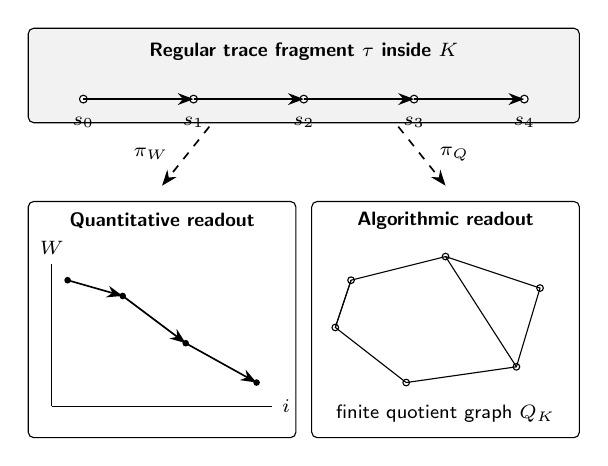
\begin{tikzpicture}[x=1mm, y=1mm, figfont]
		% Shared object: regular trace fragment
		\draw[rounded corners=2pt, fill=gray!10] (-35,10) rectangle (35,22);
		\node at (0,19) {\textbf{Regular trace fragment $\tau$ inside $K$}};
		\filldraw[fill=white] (-28,13) circle (1.4pt);
		\filldraw[fill=white] (-14,13) circle (1.4pt);
		\filldraw[fill=white] (0,13) circle (1.4pt);
		\filldraw[fill=white] (14,13) circle (1.4pt);
		\filldraw[fill=white] (28,13) circle (1.4pt);
		\draw[figarrowstrong] (-28,13) -- (-14,13);
		\draw[figarrowstrong] (-14,13) -- (0,13);
		\draw[figarrowstrong] (0,13) -- (14,13);
		\draw[figarrowstrong] (14,13) -- (28,13);
		\node[anchor=north] at (-28,12) {$s_0$};
		\node[anchor=north] at (-14,12) {$s_1$};
		\node[anchor=north] at (0,12) {$s_2$};
		\node[anchor=north] at (14,12) {$s_3$};
		\node[anchor=north] at (28,12) {$s_4$};

		% Projection arrows
		\draw[figarrowstrong, dashed] (-12,9.5) -- (-18,2);
		\draw[figarrowstrong, dashed] (12,9.5) -- (18,2);
		\node[anchor=east] at (-16,6) {$\pi_W$};
		\node[anchor=west] at (16,6) {$\pi_Q$};

		% Left panel: quantitative readout
		\draw[rounded corners=2pt] (-35,-30) rectangle (-1,0);
		\node at (-18,-2.5) {\textbf{Quantitative readout}};
		\draw (-32,-26) -- (-32,-8);
		\draw (-32,-26) -- (-4,-26);
		\node[anchor=south] at (-32,-8) {$W$};
		\node[anchor=west] at (-4,-26) {$i$};
		\fill (-30,-10) circle (1.2pt);
		\fill (-23,-12) circle (1.2pt);
		\fill (-15,-18) circle (1.2pt);
		\fill (-6,-23) circle (1.2pt);
		\draw[figarrowstrong] (-30,-10) -- (-23,-12);
		\draw[figarrowstrong] (-23,-12) -- (-15,-18);
		\draw[figarrowstrong] (-15,-18) -- (-6,-23);

		% Right panel: algorithmic readout
		\draw[rounded corners=2pt] (1,-30) rectangle (35,0);
		\node at (18,-2.5) {\textbf{Algorithmic readout}};
		\filldraw[fill=white] (6,-10) circle (1.2pt);
		\filldraw[fill=white] (18,-7) circle (1.2pt);
		\filldraw[fill=white] (30,-11) circle (1.2pt);
		\filldraw[fill=white] (27,-21) circle (1.2pt);
		\filldraw[fill=white] (13,-23) circle (1.2pt);
		\filldraw[fill=white] (4,-16) circle (1.2pt);
		\draw (6,-10) -- (18,-7) -- (30,-11) -- (27,-21) -- (13,-23) -- (4,-16) -- cycle;
		\draw (6,-10) -- (4,-16);
		\draw (18,-7) -- (27,-21);
		\node at (18,-27) {finite quotient graph $Q_K$};
	\end{tikzpicture}
	\caption{Two interpretations of one regular kernel fragment: quantitative descent and algorithmic quotient exploration.}
	\label{fig:p2-computable-dynamics-claims}
\end{figure}

Our contributions in this paper are as follows:
\begin{enumerate}
	\item A quantitative descent theorem with explicit productive-step and scheduler-lifted total-step bounds from one weighted measure.
	\item A uniform algorithmic schema that turns regular finite reachability into reusable decidability procedures.
	\item A crash-stop tolerance characterization with decision and residual-graph exactness under stated side conditions.
	\item A Byzantine safety characterization interface with exact iff form, converse counterexample families, and VM-bridge handoff obligations.
	\item A mechanized architecture that shares one regularity kernel across quantitative and algorithmic branches.
\end{enumerate}

Related liveness lines often emphasize qualitative progress in session-typed settings (Honda et al., 2008, and Caires and Pfenning, 2010). Related mechanized lines expose proof brittleness and motivate reusable proof architecture (Tirore et al., 2025).

\begin{table}[H]
	\centering
	\small
			\begin{tabularx}{\columnwidth}{@{}L{0.33\columnwidth}L{0.62\columnwidth}@{}}
			\toprule
			\thead{Symbol}         & \thead{Meaning}                      \\
			\midrule
			$\Hbyz$                & Byzantine characterization bundle    \\
			$\Obssafe$             & Byzantine safety-visible observation \\
			$\Eqsafe$              & Byzantine safety-visible equality    \\
			$\Ebyz$                & Byzantine determinism-envelope       \\
			\Coherent              & inherited operational coherence predicate \\
			$W$                    & weighted measure on state            \\
			$W_0$                  & initial weighted measure             \\
			$\Delta W$             & one-step change in weighted measure  \\
			$P(\tau)$              & productive-step count on trace $\tau$ \\
			$T(\tau)$              & total-step count on trace $\tau$     \\
			\Profile$(\sigma)$     & scheduler profile predicate          \\
			$\kappa_\sigma$        & scheduler-lift factor for profile $\sigma$ \\
			\Phase$(B)$            & low/critical/high phase at buffer level $B$ \\
			$\Bc$                  & critical capacity threshold          \\
			$\ByzChar$             & Byzantine characterization formula   \\
			$\ByzSafe$             & Byzantine safety predicate           \\
			\texttt{DeliveryModel} & parametric delivery interface        \\
			\bottomrule
		\end{tabularx}
	\caption{Notation used in this paper.}
	\label{tab:p2-notation}
\end{table}

% ============================================================================
\section{Model Summary}
\label{sec:model}
% ============================================================================

The model uses asynchronous buffered semantics with active-edge Coherence from \emph{Coherence for Asynchronous Buffered MPST}. Delivery behavior is parameterized by \texttt{DeliveryModel}.

Table~\ref{tab:p2-assumptions} records the assumptions used for exact statements in this paper.

\begin{table}[H]
	\centering
	\small
	\begin{tabularx}{\columnwidth}{@{}L{0.52\columnwidth}L{0.43\columnwidth}@{}}
		\toprule
		\thead{Assumption}          & \thead{Status}             \\
		\midrule
		async buffered semantics    & required                   \\
		active-edge Coherence       & required                   \\
		regular finite-reachability & req.\ for decidability     \\
		fairness profile            & req.\ for scheduler bounds \\
		crash-stop fault model      & req.\ for Theorem~\ref{thm:crash} \\
		Byzantine bundle $\Hbyz$    & req.\ for Thm.~\ref{thm:byzantine}, Cor.~\ref{cor:converse} \\
		\bottomrule
	\end{tabularx}
	\caption{Assumptions for exact statements.}
	\label{tab:p2-assumptions}
\end{table}

\begin{assumption}[Core Model Premises]
	\label{assump:p2-core}
	Core claims in this paper assume asynchronous buffered semantics, active-edge Coherence, regular finite reachability for decision results, and the stated fairness profile for scheduler-lifted bounds.
\end{assumption}

\begin{definition}[Productive Step]
	For the one-step transition relation $s \to s'$, a step is productive iff $W(s') < W(s)$, where $W$ is Definition~\ref{def:p2-weighted-measure}.
\end{definition}

\begin{definition}[Weighted Measure]
	\label{def:p2-weighted-measure}
	For a session state, $W = 2 \cdot \Sigma\text{depth} + \Sigma\text{buffer}$. In the mechanization this function is \texttt{weightedMeasure}.
\end{definition}

The factor two is required for strict decrease on send and select steps where one enqueue occurs. The same definition is used for global lifts and scheduler bounds.

Table~\ref{tab:p2-scheduler-profiles} lists scheduler profiles used by the bound statements.

\begin{table}[H]
	\centering
	\footnotesize
	\begin{tabularx}{\columnwidth}{@{}L{0.21\columnwidth}L{0.42\columnwidth}L{0.27\columnwidth}@{}}
		\toprule
		\thead{Profile}  & \thead{Assumption}       & \thead{Bound class} \\
		\midrule
		round-robin      & bounded delay            & total conservative  \\
		$k$-fair         & enabled within $k$ slots & total conservative  \\
		adversarial fair & fairness only            & productive exact    \\
		\bottomrule
	\end{tabularx}
	\caption{Scheduler profiles.}
	\label{tab:p2-scheduler-profiles}
\end{table}

% ============================================================================
\section{Worked Example}
\label{sec:example}
% ============================================================================

We use one running example with explicit trace witnesses.

\noindent\begingroup\raggedright
\textbf{Running example.} Protocol (as in \emph{Coherence for Asynchronous Buffered MPST}):
\par\endgroup

\noindent\begin{minipage}{\columnwidth}
	\begin{lstlisting}
C -> P : Request(n)
P -> C : Grant(k)
C -> M : Report(k)
M -> P : Confirm
P -> C : Token(t)
\end{lstlisting}
\end{minipage}

Let the initial state be $s_0$ with one pending request on edge \texttt{(C,P)} and local depths 5, 5, and 2 for \texttt{P}, \texttt{C}, and \texttt{M}. Then
\begin{equation}
	W_0 = W(s_0) = 2 \cdot (5+5+2) + 1 = 25.
\end{equation}
Assume the typing/well-formedness judgment $\Gamma \vdash s_0\ \wf$ and step judgments $s_i \to s_{i+1}$ for the trace below.

Define witness trace
\begin{equation}
	\tau_{\mathrm{ex}}: s_0 \to s_1 \to s_2 \to s_3 \to s_4.
\end{equation}
with step kinds \texttt{recv Request}, \texttt{send Grant}, \texttt{recv Grant}, \texttt{send Report}.

The quantitative facts are used through the following derivation forms.

\eqnote{Example derivation: descent}
\begingroup
\small
\begin{equation}
	\dfrac{
		\Gamma \vdash \tau_{\mathrm{ex}}: s_0 \to^\ast s_4;\ \forall i<4,\ \Delta W(s_i,s_{i+1})=-1
	}{
		W(s_4)=W_0-4=21;\ P(\tau_{\mathrm{ex}})=4\le W_0
	}
\end{equation}
\endgroup
\eqnote{Example derivation: scheduler lift}
\begin{equation}
	\dfrac{
		\Profile(\sigma);\ \kappa_\sigma=2;\ W_0=25
	}{
		\forall \tau,\ T(\tau)\le \kappa_\sigma W_0 = 50
	}
\end{equation}
\eqnote{Example derivation: phase boundary}
	\begin{equation}
		\dfrac{
		\Bc=2;\ \Phase\ \text{as in Theorem~\ref{thm:app-p2-sharp-capacity}}
		}{
			\begin{aligned}
				\Phase(1) & =\mathsf{Low}      \\
			\Phase(2) & =\mathsf{Critical} \\
			\Phase(3) & =\mathsf{High}
		\end{aligned}
	}
\end{equation}

Table~\ref{tab:p2-delta-w} records the per-rule $\Delta W$ facts used in this witness.

\begin{table}[H]
	\centering
	\small
	\begin{tabularx}{\columnwidth}{@{}L{0.65\columnwidth}>{\raggedleft\arraybackslash}p{0.30\columnwidth}@{}}
		\toprule
		\thead{Rule instance}    & $\Delta W$    \\
		\midrule
		send \texttt{Request}    & $-2 + 1 = -1$ \\
		receive \texttt{Request} & $-1$          \\
		send \texttt{Grant}      & $-2 + 1 = -1$ \\
		receive \texttt{Grant}   & $-1$          \\
		\bottomrule
	\end{tabularx}
	\caption{Per-rule $\Delta W$ facts.}
	\label{tab:p2-delta-w}
\end{table}

% ============================================================================
\section{Quantitative Dynamics}
\label{sec:theorem1}
% ============================================================================

\begin{assumption}[Quantitative Descent Premises]
	\label{assump:p2-quantitative}
	The descent theorem assumes well-typed asynchronous buffered transitions, active-edge Coherence preservation from \emph{Coherence for Asynchronous Buffered MPST}, non-negativity of $W$, and a scheduler profile from Table~\ref{tab:p2-scheduler-profiles} when total-step lifting is claimed.
\end{assumption}

\begin{theorem}[Quantitative Dynamics]
	\label{thm:quantitative}
	For any initial state $s_0$ and finite trace $\tau : s_0 \to \cdots \to s_n$ satisfying Assumption Block~\ref{assump:p2-quantitative}, let $P(\tau)$ be the productive-step count and $T(\tau)$ be the total-step count. Then
	\begin{equation}
		P(\tau) \le W(s_0) = W_0.
	\end{equation}
	If the selected scheduler profile provides lift constant $\kappa_\sigma$, then
	\begin{equation}
		T(\tau) \le \kappa_\sigma \cdot W_0.
	\end{equation}
	The productive bound is exact under the model assumptions. The scheduler-lifted bound is conservative and profile-dependent.
\end{theorem}

\begin{proof}[Proof sketch]
	Define \texttt{weightedMeasure = 2*sumDepths + sumBuffers}. First prove rule-local decrease lemmas for send/recv/select/branch (\nolinkurl{send_step_decreases},\allowbreak\ \nolinkurl{recv_step_decreases},\allowbreak\ \nolinkurl{select_step_decreases},\allowbreak\ \nolinkurl{branch_step_decreases}). Lift these to the configuration step relation using \nolinkurl{total_measure_decreasing}. Since $W \ge 0$ and each productive step decreases $W$ by at least one, productive-step count is bounded by $W_0$. Under a scheduler profile with lift constant $\kappa_\sigma$, apply the scheduler-lift theorem to obtain $T(\tau) \le \kappa_\sigma W_0$.
\end{proof}

The local decrease lemmas are \nolinkurl{send_step_decreases},\allowbreak\ \nolinkurl{recv_step_decreases},\allowbreak\ \nolinkurl{select_step_decreases}, and \nolinkurl{branch_step_decreases}. The configuration-level lift is \nolinkurl{total_measure_decreasing}.

The weighted-measure decomposition used by Theorem~\ref{thm:quantitative} is:
\begin{equation}
	\label{eq:p2-weighted-decomposition}
	\begin{array}{c}
		W(s) = 2 \cdot \Sigma\mathrm{depth}(s) + \Sigma\mathrm{buffer}(s)
		\\
			\Downarrow
			\\
			\begin{aligned}[t]
				D(s) & := \Sigma\mathrm{depth}(s);  \\
				B(s) & := \Sigma\mathrm{buffer}(s); \\
				W(s) & = 2D(s)+B(s).
			\end{aligned}
		\end{array}
\end{equation}

The rule-local descent pattern lifted to global productive-step bounds is:
\begin{equation}
	\label{eq:p2-rule-descent-table}
		\begin{array}{c|c}
			\text{productive rule family} & \text{net effect on }W
			\\
			\hline
			\text{send / select}          & \Delta W \le -1
			\\
			\text{recv / branch}          & \Delta W \le -1
		\end{array}
	\end{equation}
\begin{equation}
	\label{eq:p2-rule-descent}
	\text{therefore}\quad \Delta W \le -1\ \text{on productive steps}.
\end{equation}

% ============================================================================
\section{Algorithmic Dynamics Schema}
\label{sec:theorem2}
% ============================================================================

\begin{assumption}[Regular Finite-Reachability Premises]
	\label{assump:p2-regular}
	The decision schema assumes regularity hypotheses that produce finite reachable-state spaces and predicate reductions expressed by total decision procedures on those spaces.
\end{assumption}

\begin{theorem}[Algorithmic Dynamics Schema]
	\label{thm:algorithmic}
	For any predicate family $\mathcal{P}$ that satisfies Assumption Block~\ref{assump:p2-regular}, there exists a total decider $\mathsf{dec}_{\mathcal{P}}$ such that
	\begin{equation}
		\begin{aligned}[t]
			\forall x,\ \mathsf{dec}_{\mathcal{P}}(x) = \mathsf{true}
			\\
			\iff\ \mathcal{P}(x).
		\end{aligned}
	\end{equation}
	In particular, asynchronous subtyping and regular type equivalence are decidable on the regular fragment.
\end{theorem}

Coinductive boundary note: effect-level transport is restricted to the witness-carrying rational subclass via \nolinkurl{rationalEffect_transport_bridge}; witness-check soundness/completeness is provided by \nolinkurl{checkRationalEffectWitness_sound} and \nolinkurl{checkRationalEffectWitness_complete}; strict outside non-transportability is witnessed by \nolinkurl{strict_boundary_witness_effect}. These do not alter Theorem~\ref{thm:algorithmic} assumptions and are used in the \emph{Harmony from Coherence in Asynchronous MPST} boundary layer.

\begin{proof}[Proof sketch]
	The argument is uniform. Build finite reachable triple/pair structures from regularity (\nolinkurl{reachable_triples_finite},\allowbreak\ \nolinkurl{reachablePairs_finite}), run terminating exploration/checkers, and prove soundness/completeness for each reduction. Instantiating this schema yields deciders for async subtyping and regular equivalence (\nolinkurl{async_subtype_decidable},\allowbreak\ \nolinkurl{regularTypeEqDecide_spec}).
\end{proof}

Async subtyping instantiation appears through \nolinkurl{reachable_triples_finite} and \nolinkurl{async_subtype_decidable}. Regular type-equivalence instantiation appears through \nolinkurl{regularTypeEqCheck_sound} and \nolinkurl{regularTypeEqDecide_spec}.

Equation~\ref{eq:p2-algorithmic-workflow} records the generic workflow.
\begin{equation}
	\label{eq:p2-algorithmic-workflow}
	\begin{array}{c}
		\text{regularity assumptions}
		\\
		\Downarrow
		\\
		\text{finite reachable structure}
		\\
		\Downarrow
		\\
		\text{terminating checker } \mathsf{dec}_P
		\\
		\Downarrow
		\\
		\mathsf{dec}_P(x)=\mathsf{true}\ \Longleftrightarrow\ P(x).
	\end{array}
\end{equation}

% ============================================================================
\section{Decidability Layer}
\label{sec:decidability}
% ============================================================================

\begin{assumption}[Crash-Stop Characterization Premises]
	\label{assump:p2-crash}
	Crash-tolerance characterization assumes crash-stop faults, finite role graphs, and the residual-graph side conditions used by the decision profile.
\end{assumption}

\begin{theorem}[Crash-Stop Tolerance Characterization]
	\label{thm:crash}
	Under Assumption Block~\ref{assump:p2-crash}, there exists a total decider $\mathsf{decCrash}$ such that
	\begin{equation}
		\begin{aligned}
			\forall (R,F),\quad
			\mathsf{decCrash}(R,F) = \mathsf{true}
			\\
			\iff\ \mathsf{CrashTolerant}(R,F).
		\end{aligned}
	\end{equation}
	Moreover crash tolerance satisfies an exact residual-graph characterization:
	\begin{equation}
		\begin{aligned}[t]
			\mathsf{CrashTolerant}(R,F)
			\\
			\iff\ \mathsf{ResidualReachable}(R,F).
		\end{aligned}
	\end{equation}
	The theorem also includes witness families where topology changes flip tolerance outcomes within the stated side-condition class.
\end{theorem}

\begin{proof}[Proof sketch]
	Construct the residual graph after removing crashed roles and edges, and define \texttt{crashTolerantDec} as reachability over that residual object. Soundness is provided by \nolinkurl{crashTolerantDec_sound}, which turns a positive decider result into crash tolerance. Completeness and exact characterization come from \nolinkurl{crash_tolerance_iff}, and witness families are obtained by topology perturbations that cross the connectivity boundary.
\end{proof}

\begin{assumption}[Byzantine Characterization Premises]
	\label{assump:p2-byzantine}
	Byzantine characterization assumes explicit bundle $\Hbyz$ with fault-model, authentication and evidence-validity, conflict-exclusion primitive consistency, and adversarial-budget side conditions.
\end{assumption}

Define
\begin{equation}
	\begin{aligned}
		\ByzChar :=\; & \mathsf{ByzQuorumOK}                   \\
		              & \land \mathsf{ByzAuthEvidenceOK}       \\
		              & \land \mathsf{ByzBudgetOK}             \\
		              & \land \mathsf{ByzPrimitiveConsistent}.
	\end{aligned}
\end{equation}
where each conjunct names the corresponding requirement class in $\Hbyz$.

\begin{theorem}[Exact Byzantine Safety Characterization]
	\label{thm:byzantine}
		Under Assumption Block~\ref{assump:p2-byzantine}, profile extraction yields an exact-characterization package for the declared Byzantine model. At this paper interface, the package gives
		\begin{equation}
			\ByzChar \iff \ByzSafe.
		\end{equation}
		with relative maximality for the same characterization relation.
	\end{theorem}

\begin{proof}[Proof sketch]
	Fix the Byzantine assumption bundle as a typed profile and apply \nolinkurl{byzantineSafety_exact_of_profile} to obtain \texttt{ExactByzantineSafetyCharacterization} for the profile model.

	\begin{enumerate}
		\item Pin the Byzantine assumption bundle as a typed profile ($\Hbyz$ components).
		\item Project soundness, completeness, and maximality from the extracted exact-characterization object.
		\item Interpret soundness and completeness as the two interface implications between $\ByzChar$ and $\ByzSafe$ in this paper's model scope.
		\item Record explicit assumption classes for converse sharpness (Corollary~\ref{cor:converse}).
	\end{enumerate}

	The full envelope-maximality development is deferred to \emph{Harmony from Coherence in Asynchronous MPST}.
\end{proof}

\begin{corollary}[Converse Counterexample Families]
	\label{cor:converse}
	If any required class in $\Hbyz$ is dropped, there exists a counterexample family that violates $\ByzSafe$. The dropped classes are quorum or intersection obligations, authentication or evidence-validity obligations, adversarial-budget obligations, and primitive-consistency obligations.
\end{corollary}

\begin{proof}[Proof sketch]
	Define one constructor family per dropped assumption class in the Byzantine bundle. Each constructor forces failure of the corresponding profile obligation and induces a safety-visible violation trace. This yields class-indexed converse witnesses and therefore sharpness of Assumption Block~\ref{assump:p2-byzantine} at the safety scope stated in this paper.
\end{proof}

\begin{proposition}[Byzantine VM-Bridge Interface]
	\label{prop:vm-bridge}
	If theorem-pack capabilities include Byzantine characterization and VM envelope-adherence evidence, then runtime profile claims are constrained by $\Eqsafe$ under $\Ebyz$, and claims lacking required capability evidence are rejected by profile admission.
\end{proposition}

\begin{proof}[Proof sketch]
	The proof proceeds by capability-gated extraction. First, theorem-pack/profile APIs check the Byzantine premise bits required by the profile. Second, admitted profiles are interpreted through the VM Byzantine envelope layer, which gives the safety-visible relation $\Eqsafe$. Third, admission and conformance theorems ensure that claims without required evidence are rejected. Thus the interface is executable and proof-carrying.
\end{proof}

Core crash-tolerance lemmas include \nolinkurl{crash_tolerance_iff} and \nolinkurl{crashTolerantDec_sound}. Branching feasibility appears through \nolinkurl{branching_iff_chromatic_capacity}.

Table~\ref{tab:p2-decidability-summary} summarizes the decidability results.

\begin{table}[H]
	\centering
	\footnotesize
	\begin{tabularx}{\columnwidth}{@{}L{0.28\columnwidth}L{0.4\columnwidth}L{0.22\columnwidth}@{}}
		\toprule
		\thead{Predicate}   & \thead{Method}           & \thead{Result}  \\
		\midrule
		Async subtyping     & finite reachable triples & decidable       \\
		Regular type equiv. & finite bisim checker     & decidable       \\
		Crash-stop toler.   & residual graph decider   & decidable + iff \\
		Byzantine safety    & bundle + counterex.      & exact iff       \\
		Branching feasib.   & chromatic criterion      & decidable       \\
		\bottomrule
	\end{tabularx}
	\caption{Decidability results summary.}
	\label{tab:p2-decidability-summary}
\end{table}

Table~\ref{tab:p2-complexity-envelopes} summarizes complexity envelopes for the decision layer.

\begin{table}[H]
	\centering
	\footnotesize
	\begin{tabularx}{\columnwidth}{@{}L{0.27\columnwidth}L{0.36\columnwidth}L{0.27\columnwidth}@{}}
		\toprule
		\thead{Predicate}   & \thead{Driver}        & \thead{Complexity}   \\
		\midrule
		async subtyping     & reachable triples     & poly in graph size   \\
		regular type equiv. & finite bisim graph    & poly in graph size   \\
		crash-stop toler.   & residual connectivity & linear/near-linear   \\
		branching feasib.   & coloring checks       & poly for fixed prof. \\
		\bottomrule
	\end{tabularx}
	\caption{Complexity envelopes.}
	\label{tab:p2-complexity-envelopes}
\end{table}

% ============================================================================
\section{Quantitative Corollaries}
\label{sec:corollaries}
% ============================================================================

\begin{corollary}[Productive-Step Bound]
	\label{cor:productive}
	For any trace $\tau$ satisfying Assumption Block~\ref{assump:p2-quantitative}, $P(\tau) \le W_0$.
\end{corollary}

\begin{corollary}[Scheduler-Lifted Total Bound]
	\label{cor:scheduler}
	For any trace $\tau$ satisfying Assumption Block~\ref{assump:p2-quantitative} and scheduler profile $\sigma$ with lift constant $\kappa_\sigma$, $T(\tau) \le \kappa_\sigma \cdot W_0$.
\end{corollary}

\begin{corollary}[Critical Capacity Boundary]
	\label{cor:capacity}
	There exists a computable threshold $\Bc$ such that the declared phase classifier over buffer capacity is exact at the theorem interface under the stated assumptions.
\end{corollary}

\begin{proof}[Proof sketch]
	Corollary~\ref{cor:productive} is the first clause of Theorem~\ref{thm:quantitative} with notation specialized to productive-step count. Instantiating Theorem~\ref{thm:quantitative} at the same trace and premises yields the stated inequality directly.
\end{proof}

\begin{proof}[Proof sketch]
	Corollary~\ref{cor:scheduler} is the scheduler-lift clause of Theorem~\ref{thm:quantitative} with the same premises and profile constant $\kappa_\sigma$. Substituting the selected scheduler profile into that clause yields the stated bound.
\end{proof}

\begin{proof}[Proof sketch]
	\nolinkurl{critical_buffer_computable} provides existence of a computable boundary value $\Bc$, and \nolinkurl{phase_transition_sharp} proves exact classifier behavior on each side of that boundary. Composing these two lemmas yields the stated theorem-level threshold characterization.
\end{proof}

Table~\ref{tab:p2-exact-vs-conservative} separates exact and conservative consequences.

\begin{table}[H]
	\centering
	\small
	\begin{tabularx}{\columnwidth}{@{}L{0.70\columnwidth}L{0.25\columnwidth}@{}}
		\toprule
		\thead{Result}                    & \thead{Class} \\
		\midrule
		productive-step decrease          & exact         \\
		productive-step bound by $W_0$    & exact         \\
		scheduler-lifted total-step bound & conservative  \\
		threshold under scheduler profile & conservative  \\
		\bottomrule
	\end{tabularx}
	\caption{Exact vs conservative results.}
	\label{tab:p2-exact-vs-conservative}
\end{table}

Table~\ref{tab:p2-worked-values} gives worked values used in the worked example.

\begin{table}[H]
	\centering
	\small
	\begin{tabularx}{\columnwidth}{@{}L{0.70\columnwidth}>{\raggedleft\arraybackslash}p{0.25\columnwidth}@{}}
		\toprule
		\thead{Quantity}        & \thead{Value} \\
		\midrule
		$W_0$                   & 25            \\
		productive-step bound   & $\leq 25$     \\
		2-fair total-step bound & $\leq 50$     \\
		$\Bc$                   & 2             \\
		\bottomrule
	\end{tabularx}
	\caption{Worked example values.}
	\label{tab:p2-worked-values}
\end{table}

Equation~\ref{eq:p2-phase-boundary} locates the worked example on the phase boundary.
\begin{equation}
	\label{eq:p2-phase-boundary}
	\begin{array}{c}
		\begin{aligned}[t]
			B<\Bc & \Rightarrow \Phase(B)=\mathsf{Low},      \\
			B=\Bc & \Rightarrow \Phase(B)=\mathsf{Critical}, \\
			B>\Bc & \Rightarrow \Phase(B)=\mathsf{High}.
		\end{aligned}
		\\[2pt]
		\text{worked instance: } \Bc=2,\ W_0=25,\ B=\Bc.
	\end{array}
\end{equation}
With $\Bc=2$ and $W_0=25$, the instance sits at the critical capacity line, so productive-step and scheduler-lift conclusions apply exactly as in Theorem~\ref{thm:quantitative} and Corollaries~\ref{cor:productive}--\ref{cor:scheduler}.

% ============================================================================
\section{Proof Architecture}
\label{sec:architecture}
% ============================================================================

The architecture has one shared regularity kernel and two proof branches.

\begin{itemize}
	\item quantitative branch: local-step algebra to strict descent to global bounds
	\item algorithmic branch: regularity to finite reachability to predicate decisions
\end{itemize}

This reuse reduces theorem fragmentation and proof duplication. It also gives a direct map from assumptions to output guarantees.

Dependency sketch:
\begin{enumerate}
	\item Assumption Block~\ref{assump:p2-quantitative} gives Theorem~\ref{thm:quantitative} and Corollaries~\ref{cor:productive}--\ref{cor:scheduler}.
	\item Assumption Block~\ref{assump:p2-regular} gives Theorem~\ref{thm:algorithmic} and the subtyping/equivalence deciders.
	\item Assumption Block~\ref{assump:p2-crash} gives Theorem~\ref{thm:crash}.
	\item Assumption Block~\ref{assump:p2-byzantine} gives Theorem~\ref{thm:byzantine}, Corollary~\ref{cor:converse}, and Proposition~\ref{prop:vm-bridge}.
\end{enumerate}

% ============================================================================
\section{Mechanization Summary}
\label{sec:mechanization}
% ============================================================================

Table~\ref{tab:p2-claim-artifact-map} maps claim families to concrete modules and theorem anchors.
Module references use path identifiers of the form \texttt{P$n$-A$xx$}, where $n$ is the paper number and $xx$ is the artifact index; these resolve to file paths in Appendix~\ref{app:p2-path-registry}.

\begin{table}[H]
	\centering
	\footnotesize
		{\setlength{\tabcolsep}{3pt}
		\begin{tabularx}{\columnwidth}{@{}L{0.19\columnwidth}L{0.27\columnwidth}>{\raggedright\arraybackslash}X@{}}
		\toprule
		\thead{Layer} & \thead{Modules}                               & \thead{Anchors}                                          \\
		\midrule
		Weighted dyn. & \pathref{P2-A01},\allowbreak \pathref{P2-A02} & \texttt{weightedMeasure},\allowbreak\ \nolinkurl{total_measure_decreasing} \\
			Decision      & \pathref{P2-A03},\allowbreak \pathref{P2-A04} & \nolinkurl{reachable_triples_finite},\allowbreak\ \nolinkurl{async_subtype_decidable},\newline \nolinkurl{regularTypeEqDecide_spec} \\
			Protocol      & \pathref{P2-A05},\allowbreak \pathref{P2-A06} & \nolinkurl{crash_tolerance_iff},\allowbreak\ \nolinkurl{branching_iff_chromatic_capacity},\newline \nolinkurl{phase_transition_sharp} \\
			Byzantine     & \pathref{P2-A07},\allowbreak \pathref{P2-A08} & \nolinkurl{byzantineSafety_exact_of_profile},\newline \texttt{canOperateUnder}\allowbreak\texttt{Byzantine}\allowbreak\texttt{Envelope} \\
		\bottomrule
	\end{tabularx}
	}
	\caption{Claim to artifact mapping.}
	\label{tab:p2-claim-artifact-map}
\end{table}

\begin{proposition}[Mechanization Coverage Soundness]
	\label{prop:coverage}
	For any claim class $c$ in Table~\ref{tab:p2-claim-artifact-map}, if $c$ is marked covered and the corresponding Appendix~\ref{app:reproducibility} checks pass, then there exists a mechanized theorem object for $c$ within this paper's assumption scope.
\end{proposition}

\begin{proof}[Proof sketch]
	Coverage labels in Table~\ref{tab:p2-claim-artifact-map} are defined by explicit module-and-theorem anchors. Appendix~\ref{app:reproducibility} rebuild checks certify that these declarations resolve and typecheck under the pinned toolchain. Therefore a passing check witnesses existence of a theorem object for each covered claim class.
\end{proof}

% ============================================================================
\section{Related Work}
\label{sec:related}
% ============================================================================

Classical MPST work established session foundations together with global coherence and projectability
discipline (Honda et al., 2008; Honda et al., 2016; Castagna et al., 2012). Projection refinements and local-first compatibility contrasts were developed in later lines
(Majumdar et al., 2021; Scalas and Yoshida, 2018). Logical coherence lines interpret multiparty
compatibility as n-ary duality and proof compatibility (Carbone et al., 2015; Carbone et al., 2016;
Carbone et al., 2017), and data-certification extensions remained in the same global-projection
discipline (Toninho and Yoshida, 2017). Logical formulations connect sessions and propositions and
motivate compositional proof interfaces (Caires and Pfenning, 2010, and Wadler, 2012). Program-logical
and mechanized lines expanded the verification space (Hinrichsen et al., 2020; Tirore et al., 2025). Event-structure and partial-order approaches give alternate macro views of
concurrency (Castellan et al., 2023).

On the quantitative side, our use of descent functions follows the classical drift and stochastic-stability lineage (Lyapunov, 1892; Foster, 1953; Meyn and Tweedie, 2009). On the algorithmic side, the finite-reachability posture follows communicating-automata and model-checking lines (Brand and Zafiropulo, 1983; Baier and Katoen, 2008). Fault-side interfaces are compatible with standard crash and Byzantine theory baselines (Fischer et al., 1985; Chandra and Toueg, 1996; Lamport et al., 1982; Castro and Liskov, 1999).

This paper differs in structure. It unifies quantitative bounds and algorithmic decidability through one regularity kernel. The result is a single reusable theorem program instead of isolated predicate proofs.

% ============================================================================
\section{Limitations and Scope}
\label{sec:limitations}
% ============================================================================

Quantitative bounds require the Assumption Block~\ref{assump:p2-quantitative} premises: well-typed asynchronous buffered transitions, active-edge Coherence preservation, non-negativity of $W$, and an explicit scheduler profile when total-step lifting is claimed. Scheduler-lifted totals remain conservative profile-dependent bounds rather than exact universal runtime counts.

Crash-stop characterization is exact only under Assumption Block~\ref{assump:p2-crash}, with crash-stop faults, finite role graph, and residual-graph side conditions. Byzantine results are exact safety characterizations only under Assumption Block~\ref{assump:p2-byzantine}, with $\Hbyz$ fault-model, authentication and evidence-validity, conflict-exclusion primitive consistency, and adversarial-budget side conditions, and they do not imply Byzantine liveness.

Decidability and finite exploration require the Assumption Block~\ref{assump:p2-regular} regular finite-reachability premises. Non-regular fragments and stronger adversarial models require different constructions.

Reconfiguration commutation and envelope maximality claims are out of scope for this paper and handled separately in the series.

% ============================================================================
\section{Conclusion}
\label{sec:conclusion}
% ============================================================================

This paper turns Coherence-preserving dynamics into computable dynamics. Quantitative bounds and decision procedures come from the same regularity source. That result provides the computational bridge between \emph{Coherence for Asynchronous Buffered MPST} and the reconfiguration and envelope claims in \emph{Harmony from Coherence in Asynchronous MPST}.

Byzantine contribution in this paper is the exact safety-characterization interface and converse counterexample family packaging. Byzantine liveness beyond the stated assumptions remains open and is tracked as future work.

% ============================================================================
\section*{Works Cited}
% ============================================================================

\begin{citelist}
	\item Baier, C., and Katoen, J.-P. (2008). Principles of Model Checking. MIT Press.
	\item Brand, D., and Zafiropulo, P. (1983). On Communicating Finite-State Machines. Journal of the ACM, 30(2), 323--342.
	\item Caires, L., and Pfenning, F. (2010). Session Types as Intuitionistic Linear Propositions. CONCUR 2010.
	\item Carbone, M., Lindley, S., Montesi, F., Sch\"urmann, C., and Wadler, P. (2016). Coherence Generalises Duality: A Logical Explanation of Multiparty Session Types. CONCUR 2016.
	\item Carbone, M., Montesi, F., Sch\"urmann, C., and Yoshida, N. (2015). Multiparty Session Types as Coherence Proofs. CONCUR 2015.
	\item Carbone, M., Montesi, F., Sch\"urmann, C., and Yoshida, N. (2017). Multiparty Session Types as Coherence Proofs. Acta Informatica, 54(3), 243--269.
	\item Castagna, G., Dezani-Ciancaglini, M., Gesbert, N., and Padovani, L. (2012). On Global Types and Multi-Party Sessions.
	\item Castellan, S., et al. (2023). Event-structure and partial-order semantics for session-based concurrency. Journal of Logic and Algebraic Methods in Programming.
	\item Castro, M., and Liskov, B. (1999). Practical Byzantine Fault Tolerance. OSDI 1999.
	\item Chandra, T. D., and Toueg, S. (1996). Unreliable Failure Detectors for Reliable Distributed Systems. Journal of the ACM, 43(2), 225--267.
	\item Cover, T. M., and Thomas, J. A. (2006). Elements of Information Theory (2nd ed.). Wiley.
	\item Dwork, C., Lynch, N., and Stockmeyer, L. (1988). Consensus in the Presence of Partial Synchrony. Journal of the ACM, 35(2), 288--323.
	\item Fischer, M. J., Lynch, N. A., and Paterson, M. S. (1985). Impossibility of Distributed Consensus with One Faulty Process. Journal of the ACM, 32(2), 374--382.
	\item Foster, F. G. (1953). On the stochastic matrices associated with certain queueing processes. Annals of Mathematical Statistics, 24(3), 355--360.
	\item Hinrichsen, J., et al. (2020). Actris: Session-type based reasoning in separation logic. POPL 2020.
	\item Honda, K., Yoshida, N., and Carbone, M. (2008). Multiparty Asynchronous Session Types. POPL 2008.
	\item Honda, K., Yoshida, N., and Carbone, M. (2016). Multiparty Asynchronous Session Types. Journal of the ACM, 63(1), Article 9.
	\item Hopcroft, J. E., and Ullman, J. D. (1979). Introduction to Automata Theory, Languages, and Computation. Addison-Wesley.
	\item Karp, R. M., and Miller, R. E. (1969). Parallel Program Schemata. Journal of Computer and System Sciences, 3(2), 147--195.
	\item Lamport, L., Shostak, R., and Pease, M. (1982). The Byzantine Generals Problem. ACM Transactions on Programming Languages and Systems, 4(3), 382--401.
	\item Majumdar, R., Mukund, M., Stutz, F., and Zufferey, D. (2021). Generalising Projection in Asynchronous Multiparty Session Types. CONCUR 2021.
	\item Lynch, N. A. (1996). Distributed Algorithms. Morgan Kaufmann.
	\item Lyapunov, A. M. (1892). The General Problem of the Stability of Motion. Kharkov Mathematical Society.
	\item Meyn, S. P., and Tweedie, R. L. (2009). Markov Chains and Stochastic Stability (2nd ed.). Cambridge University Press.
	\item Scalas, A., and Yoshida, N. (2018). Multiparty Session Types, Beyond Duality. Journal of Logical and Algebraic Methods in Programming, 97, 55--84.
	\item Shannon, C. E. (1948). A Mathematical Theory of Communication. Bell System Technical Journal, 27(3), 379--423 and 27(4), 623--656.
	\item Tirore, L., Bengtson, J., and Carbone, M. (2025). Mechanized MPST metatheory with subject-reduction robustness analysis. ECOOP 2025.
	\item Toninho, B., and Yoshida, N. (2017). Certifying Data in Multiparty Session Types. Journal of Logical and Algebraic Methods in Programming, 90, 61--83.
	\item Wadler, P. (2012). Propositions as Sessions. ICFP 2012.
\end{citelist}

% ============================================================================
\clearpage
\appendix
\noindent{\Large\bfseries Appendix}
\vspace{0.5em}
% ============================================================================

\section{Deferred Quantitative Proofs}
\label{app:quantitative}

This appendix expands Theorem~\ref{thm:quantitative} and Corollaries~\ref{cor:productive}--\ref{cor:scheduler}.

\subsection{Weighted Potential and Productive Steps}

For local state $s$, define:

\noindent\begin{minipage}{\columnwidth}
	\begin{lstlisting}
W(s) := 2 * sumDepths(s) + sumBuffers(s)
\end{lstlisting}
\end{minipage}

For global configuration $C$, write $W(C)$ for the sum of local/session contributions. A step is productive iff it decreases $W$ strictly.

\subsection{Rule-Level Decrease}

\begin{lemma}[Send/Select Decrease]
	\label{lem:app-p2-send-select}
	For productive send/select steps, $\Delta W \le -1$.
\end{lemma}

\begin{proof}[Proof sketch]
	Unfold the weighted measure into depth and buffer components. A productive send or select step consumes one protocol constructor, contributing $-2$ to depth, and enqueues at most one message, contributing $+1$ to buffers. Summing contributions gives $\Delta W \le -1$.
\end{proof}

\begin{lemma}[Recv/Branch Decrease]
	\label{lem:app-p2-recv-branch}
	For productive recv/branch steps, $\Delta W \le -1$.
\end{lemma}

\begin{proof}[Proof sketch]
	For productive recv and branch steps, one buffered head is consumed and no new message is enqueued on that edge. Unfolding the weighted accounting shows a strict negative contribution from the consumed buffer and continuation progress. Therefore $\Delta W \le -1$.
\end{proof}

\begin{lemma}[Configuration Lift]
	\label{lem:app-p2-config-lift}
	Rule-level decreases lift to the global step relation:

	\noindent\begin{minipage}{\columnwidth}
		\begin{lstlisting}
productiveStep C C' -> W(C') <= W(C) - 1
\end{lstlisting}
	\end{minipage}
\end{lemma}

\begin{proof}[Proof sketch]
	Decompose the global step into updated and untouched local components. Apply Lemma~\ref{lem:app-p2-send-select} or Lemma~\ref{lem:app-p2-recv-branch} on updated components and use zero change on untouched components. Summing all contributions yields the stated inequality.
\end{proof}

\subsection{Trace Bounds}

\begin{proposition}[Productive-Step Bound]
	\label{prop:app-p2-productive-bound}
	For any finite trace from $C_0$, productive-step count $P$ satisfies $P \le W(C_0)$.
\end{proposition}

\begin{proof}[Proof sketch]
	Index productive positions in the trace and apply Lemma~\ref{lem:app-p2-config-lift} at each such index. Summing inequalities telescopes to $W(C_0) - W(C_n) \ge P$. Since $W(C_n) \ge 0$, we conclude $P \le W(C_0)$.
\end{proof}

\begin{proposition}[Scheduler-Lifted Total Bound]
	\label{prop:app-p2-scheduler-bound}
	If scheduler profile $\sigma$ admits lift constant $\kappa_\sigma$, then total steps $T$ satisfy:
	\begin{equation}
		T \le \kappa_\sigma \cdot W(C_0).
	\end{equation}
\end{proposition}

\begin{proof}[Proof sketch]
	Proposition~\ref{prop:app-p2-productive-bound} bounds the number of productive steps by $W(C_0)$. The scheduler profile contributes a bound on how many non-productive steps can occur between productive ones. Multiplying these bounds gives $T \le \kappa_\sigma \cdot W(C_0)$.
\end{proof}

Theorem~\ref{thm:quantitative} and Corollaries~\ref{cor:productive}--\ref{cor:scheduler} are exactly Propositions~\ref{prop:app-p2-productive-bound}--\ref{prop:app-p2-scheduler-bound} under Assumption Block~\ref{assump:p2-quantitative}.

\section{Deferred Proof of Algorithmic Decidability Schema}
\label{app:algorithmic}

\subsection{Abstract Schema}

Let $P$ be a predicate over inputs $x$. Assume:
\begin{enumerate}
	\item a finite reachable structure $\mathrm{Reach}(x)$,
	\item a terminating checker $\mathrm{check}(x)$ over $\mathrm{Reach}(x)$,
	\item soundness/completeness: $\mathrm{check}(x) = \mathsf{true} \Leftrightarrow P(x)$.
\end{enumerate}

\begin{theorem}[Generic Decider Transfer]
	Under the three assumptions above, $P$ is decidable.
\end{theorem}

\begin{proof}[Proof sketch]
	Finiteness of $\mathrm{Reach}(x)$ ensures that exploration terminates. The soundness and completeness hypotheses identify $\mathrm{check}(x)$ with truth of $P(x)$. Therefore the checker is a total decision procedure for $P$.
\end{proof}

\subsection{Complexity Envelope (Schema Level)}

Let $N(x)$ be size of the finite reachable object. If check runs in $\mathrm{poly}(N(x))$, then decision complexity is $\mathrm{poly}(N(x))$.

This explains why the paper reports complexity in explored-graph size, not in raw syntax size.

\subsection{Instantiations}

\begin{enumerate}
	\item Async subtyping: reachable triple graph (\nolinkurl{reachable_triples_finite},\allowbreak\ \nolinkurl{async_subtype_decidable}).
	\item Regular equivalence: reachable pair/bisim graph (\nolinkurl{regularTypeEqCheck_sound},\allowbreak\ \nolinkurl{regularTypeEqDecide_spec}).
\end{enumerate}

\section{Instantiated Decision Theorems}
\label{app:instantiated}

\subsection{Crash-Stop Tolerance Instantiation}

Given role graph $R$ and crash set $F$, let $\mathrm{Residual}(R,F)$ remove crashed roles and incident edges.

\begin{theorem}[Crash-Stop Exactness]
	\label{thm:app-p2-crash-exactness}
	\begin{equation}
		\begin{aligned}[t]
			\mathsf{CrashTolerant}(R,F)
			\\
			\iff\ \mathsf{ResidualReachable}(R,F).
		\end{aligned}
	\end{equation}
\end{theorem}

\begin{proof}[Proof sketch]
	For soundness, if the residual graph is disconnected then at least one required communication path is cut, so crash tolerance fails. For completeness, residual reachability gives continuation witnesses for all required communication obligations in the crash-stop model. Combining both directions yields the claimed equivalence.
\end{proof}

\subsection{Branching Feasibility Instantiation}

Let \texttt{ConfGraph} be the confusability graph induced by branch-distinguishability constraints.

\begin{theorem}[Branching Feasibility Criterion]
	\label{thm:app-p2-branching}
	Feasibility holds iff the declared chromatic-capacity condition on \texttt{ConfGraph} holds.
\end{theorem}

\begin{proof}[Proof sketch]
	Encode branch distinguishability constraints as coloring constraints on \texttt{ConfGraph}. The profile fixes admissible class counts, so feasibility reduces to existence of a coloring within that bound. The equivalence follows by bidirectional translation between branch witnesses and valid colorings.
\end{proof}

\subsection{Capacity Threshold Instantiation}

Define the phase classifier
\begin{equation}
	\Phase(B) =
	\begin{cases}
		\mathsf{Low},      & B < \Bc, \\
		\mathsf{Critical}, & B = \Bc, \\
		\mathsf{High},     & B > \Bc.
	\end{cases}
\end{equation}
	\begin{theorem}[Sharp Capacity Boundary]
		\label{thm:app-p2-sharp-capacity}
			There exists a computable threshold $\Bc$ such that
			\begin{equation}
				\begin{aligned}[t]
					\forall B,\quad
					&(B < \Bc \Rightarrow \Phase(B)=\mathsf{Low}) \\
					&\land (B = \Bc \Rightarrow \Phase(B)=\mathsf{Critical}) \\
					&\land (B > \Bc \Rightarrow \Phase(B)=\mathsf{High}).
				\end{aligned}
			\end{equation}
			with exactness at the theorem interface.
		\end{theorem}

\begin{proof}[Proof sketch]
	\nolinkurl{critical_buffer_computable} yields a computable candidate threshold. \nolinkurl{phase_transition_sharp} proves that the classifier is exact below, at, and above this threshold. Therefore the phase boundary is both computable and sharp.
\end{proof}

\subsection{Byzantine Safety Interface (Scope of This Paper)}

Under Assumption Block~\ref{assump:p2-byzantine}, this paper provides the exact safety-side interface and converse counterexample packaging; full envelope maximality and transport are deferred to \emph{Harmony from Coherence in Asynchronous MPST}.

\section{Mechanization Map}
\label{app:mechanization}

\begin{table}[H]
	\centering
	\footnotesize
		{\setlength{\tabcolsep}{3pt}
		\begin{tabularx}{\columnwidth}{@{}L{0.23\columnwidth}L{0.25\columnwidth}>{\raggedright\arraybackslash}X@{}}
		\toprule
		\thead{Result}   & \thead{Modules}                               & \thead{Anchors}                      \\
		\midrule
		Quant.\ dynamics & \pathref{P2-A01},\allowbreak \pathref{P2-A02} & \texttt{weightedMeasure},\allowbreak\ \nolinkurl{total_measure_decreasing} \\
			Decidability     & \pathref{P2-A03},\allowbreak \pathref{P2-A04} & \nolinkurl{reachable_triples_finite},\allowbreak\ \nolinkurl{async_subtype_decidable},\newline \nolinkurl{regularTypeEqDecide_spec} \\
			Crash/branch     & \pathref{P2-A05},\allowbreak \pathref{P2-A06} & \nolinkurl{crash_tolerance_iff},\allowbreak\ \nolinkurl{branching_iff_chromatic_capacity},\newline \nolinkurl{phase_transition_sharp}      \\
			Byzantine        & \pathref{P2-A07},\allowbreak \pathref{P2-A08} & \nolinkurl{byzantineSafety_exact_of_profile},\newline \texttt{canOperateUnder}\allowbreak\texttt{Byzantine}\allowbreak\texttt{Envelope}    \\
		\bottomrule
	\end{tabularx}
	}
	\caption{Mechanization map.}
	\label{tab:p2-mechanization-map}
\end{table}

\section{Artifact Path Registry}
\label{app:p2-path-registry}

All Lean file-path references in this paper use the identifiers listed in Table~\ref{tab:p2-path-registry}.

\begin{table}[H]
	\centering
	\footnotesize
	\begin{tabularx}{\columnwidth}{@{}L{0.2\columnwidth}L{0.75\columnwidth}@{}}
		\toprule
		\thead{ID}      & \thead{Path (relative to \texttt{lean/})}                          \\
		\midrule
		\texttt{P2-A01} & \texttt{Runtime/\allowbreak Proofs/\allowbreak WeightedMeasure/\allowbreak}\mbox{\texttt{*.lean}}                   \\
		\texttt{P2-A02} & \texttt{Runtime/\allowbreak Proofs/\allowbreak}\mbox{\texttt{Lyapunov.lean}}                            \\
		\texttt{P2-A03} & \texttt{SessionCoTypes/\allowbreak AsyncSubtyping/\allowbreak}\mbox{\texttt{*.lean}}                    \\
		\texttt{P2-A04} & \texttt{SessionCoTypes/\allowbreak Coinductive/\allowbreak BisimDecidable/\allowbreak}\mbox{\texttt{*.lean}}        \\
		\texttt{P2-A05} & \texttt{Protocol/\allowbreak}\mbox{\texttt{CrashTolerance.lean}}                            \\
		\texttt{P2-A06} & \texttt{Protocol/\allowbreak BufferBoundedness/\allowbreak}\mbox{\texttt{PhaseSharpness.lean}}          \\
		\texttt{P2-A07} & \texttt{Runtime/\allowbreak Proofs/\allowbreak Adapters/\allowbreak Distributed/\allowbreak}\mbox{\texttt{EnvelopeTheorems.lean}} \\
		\texttt{P2-A08} & \texttt{Runtime/\allowbreak Proofs/\allowbreak TheoremPack/\allowbreak}\mbox{\texttt{*.lean}}                       \\
		\bottomrule
	\end{tabularx}
	\caption{Artifact path registry for \emph{Computable Dynamics for Asynchronous MPST}.}
	\label{tab:p2-path-registry}
\end{table}

\section{Exactness and Boundary Notes}
\label{app:exactness}

\subsection{Exact Claims}

\begin{enumerate}
	\item Productive-step decrease and productive-step bounds (Assumption Block~\ref{assump:p2-quantitative}).
	\item Crash-stop characterization (Assumption Block~\ref{assump:p2-crash}).
	\item Byzantine safety characterization at paper interface scope (Assumption Block~\ref{assump:p2-byzantine}).
\end{enumerate}

\subsection{Conservative or Profile-Indexed Claims}

\begin{enumerate}
	\item Scheduler-lifted total-step bounds ($\kappa_\sigma$-indexed).
	\item Complexity bounds parameterized by explored finite-state size.
	\item Capacity-boundary reporting when profile assumptions fix classifier semantics.
\end{enumerate}

\subsection{Out-of-Scope}

\begin{enumerate}
	\item Non-regular fragments for decision transfer.
	\item Byzantine liveness under weaker timing/adversary assumptions.
	\item Reconfiguration commutation and envelope maximality (\emph{Harmony from Coherence in Asynchronous MPST}).
\end{enumerate}

\section{Reproducibility}
\label{app:reproducibility}

Reproduction uses the pinned Lean toolchain and manifest.

\begin{enumerate}
	\item Build module families listed in Appendix~\ref{app:mechanization}.
	\item Run \texttt{just escape} and \texttt{just verify-protocols}.
	\item Confirm Appendix~\ref{app:mechanization} theorem anchors resolve and typecheck.
\end{enumerate}

Expected checks: Finite-reachability and decision modules compile, weighted-measure descent and scheduler modules compile, crash and branching and threshold modules compile, and theorem-pack and profile-bridge modules compile.

\section{Index of Main Results}
\label{app:index}

\begin{table}[H]
	\centering
	\footnotesize
	{\setlength{\tabcolsep}{3pt}
	\begin{tabularx}{\columnwidth}{@{}L{0.22\columnwidth}L{0.09\columnwidth}L{0.33\columnwidth}L{0.27\columnwidth}@{}}
		\toprule
		\thead{Claim} & \thead{Sec.} & \thead{Assumption}                   & \thead{Location}      \\
		\midrule
		Thm.~\ref{thm:quantitative}    & \S4 & Assump.~\ref{assump:p2-quantitative} & \pathref{P2-A01} \\
		Thm.~\ref{thm:algorithmic}     & \S5 & Assump.~\ref{assump:p2-regular}      & \pathref{P2-A03} \\
			Thm.~\ref{thm:crash}           & \S6 & Assump.~\ref{assump:p2-crash}        & \pathref{P2-A05} \\
			Thm.~\ref{thm:byzantine}       & \S6 & Assump.~\ref{assump:p2-byzantine}    & \pathref{P2-A07} \\
			Cor.~\ref{cor:converse}        & \S6 & Thm.~\ref{thm:byzantine} + dropped class & \pathref{P2-A07} \\
			Cor.~\ref{cor:productive}      & \S7 & Thm.~\ref{thm:quantitative} premises & \pathref{P2-A01} \\
			Cor.~\ref{cor:scheduler}       & \S7 & Thm.~\ref{thm:quantitative} + sched. & \pathref{P2-A02} \\
			Cor.~\ref{cor:capacity}        & \S7 & regular + threshold assumptions       & \pathref{P2-A06}  \\
			Thm.~\ref{thm:app-p2-branching} & App.\ C & regular + branch profile & \pathref{P2-A06} \\
			Prop.~\ref{prop:vm-bridge}     & \S6 & pack + adherence                      & \pathref{P2-A08}  \\
			Prop.~\ref{prop:coverage}      & \S9 & claim-map + App.~\ref{app:reproducibility} checks & \S9 \\
		\bottomrule
	\end{tabularx}
	}
	\caption{Index of main results.}
	\label{tab:p2-index}
\end{table}

\end{document}
